\clearpage
\pagenumbering{arabic}
\chapter{Introduction}
\section{XFEL}
The world’s first free electron laser of hard X-rays, which has been built in Stanford, is called the Linac Coherent Light Source. It is a 4th generation X-ray source of ultra-short pulses of hard X-rays \cite{LCLS} built on the site of now abandoned instrumentation for particle physics. A capability of the XFEL is that it can create X-rays ten billion times brighter than those available before by any man-made source on earth delivered at the rate of 120 pulses per second. Since some crucial proteins such as membrane proteins are very difficult to crystallize, they may be forever be outside the scope of traditional X-ray crystallography. However, the unprecedented brightness of the XFEL may allow the possibility of structural solution from individual uncrystallized biomolecules. The theory developed in this dissertation is an attempt to develop theoretical methods for this precise problem. While with the vast majority of algorithms developed for this task proceed by finding the relative orientations of the molecules giving rise to the diffraction patterns it should be stressed that a relative angle is significant only if all molecules in the sample remain fixed relative to each other or else if one had only a single molecule contributing to a diffraction pattern. In reality if the molecules are presented to the X-ray beam in droplets over the course of several hours it is most likely different molecules will have changes to their orientations randomly as a consequence of molecular diffusion. The only thing that will stay constant is the molecular structure, and hence the molecular electron density. We will show that even in such cases we can deduce this structure from its angular correlations.

Think of a single particle. The integral of its angular correlations over all orientations will remain the same despite their possible different initial orientations, since they are an integral over all orientations the particle can have. Note this does not necessarily assume the particles are distributed evenly in angle. Even if particular orientations are favored, the sum of the orientations over all angles must be the same. Even if one had an ensemble of randomly oriented particles by the time one integrates over all orientations of the individual particles the contribution from each particle will be identical - its just that the sum over different orientations is done in a different order - the sum over all possible orientations is identical. Consequently, if one sums over all diffraction patterns measured in an XFEL each molecule will have an identical contribution. One may call this the angular correlation function. Consequently, if one has a method for deducing a structure from its angular correlations it would work equally well from all randomly oriented particles, independent of their orientations of a particle in an individual diffraction pattern.

The problem is that the deduction of a particle’s structure from its angular correlation function may be more difficult than its deduction from a single particle diffraction pattern, something that is well established nowadays by so-called iterative phasing programs. Its worth digressing a little to iterative phasing algorithms to understand this point. Due to the lack of phase information in measured intensities it is difficult to reconstruct a real-space density. However, there is no problem with going the other way. That us to say if one assumes an electron density one can always calculate a set of amplitudes by Fourier transforming the density and a set of intensities by taking the square moduli of the amplitudes. The idea then is to apply constraints in real and reciprocal space to the same function or its Fourier transform to constrain that function. In ordinary phasing algorithms the reciprocal space constraint is the intensity and the real space constraint is the “support” or approximate extent of the electron density that may be known a priori. A normal phasing algorithm operates in a space described by a Cartesian coordinate system. In the XFEL problem, however the particles are presented to the beam in all possible orientations. Consequently, it is more appropriate to use polar coordinates. The reciprocal space constraints in this case is to the correlations. It is possible to write the correlations in terms in of the coefficients of the spherical harmonic expansion coefficients of the diffraction volume. Consequently provided one works in a spherical harmonic system, there is not much difference to a phasing algorithm that constrains to an intensity in reciprocal space and one that constrains to a set of correlations. The real space constraint can remain the same “support” constraint as before. This is the essential idea behind the iterative phasing algorithm from the correlations proposed by Donatelli, Zwart, and Sethian in 2015 \cite{Donatelli}. As an indication of its effectiveness, we show in the figures below, the electron density of the biomolecule directly from its PDB file in the left column and its reconstruction from the intensity correlations on the right. Obviously, the algorithm is really effective in performing the reconstruction. 

\begin{figure}[ht]
  \centering
  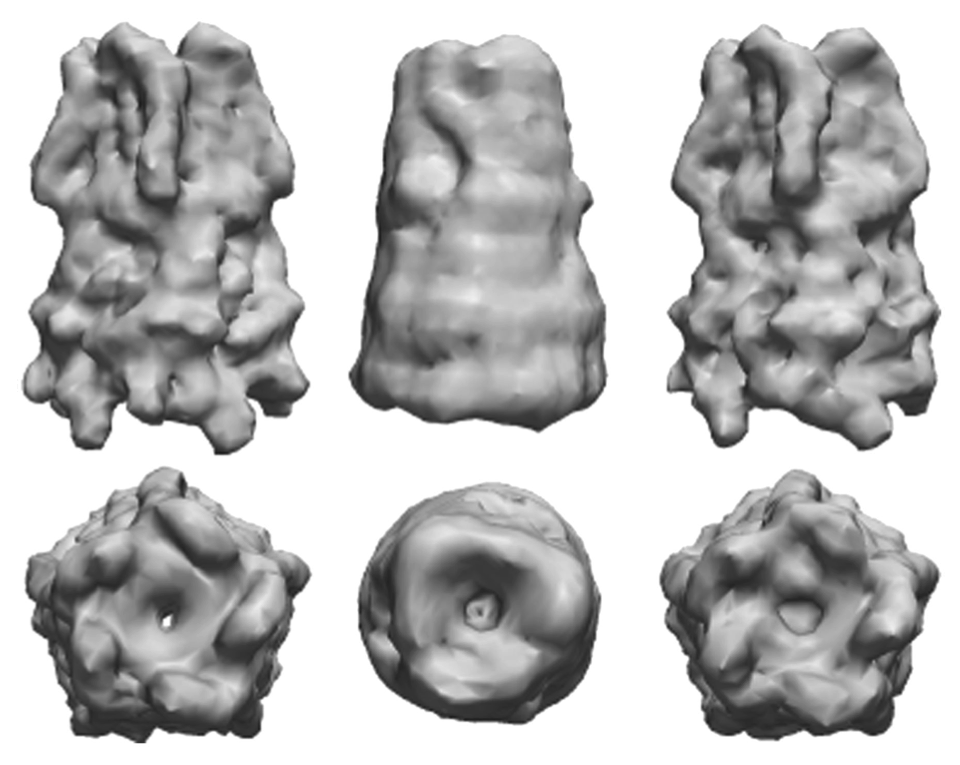
\includegraphics[width=.9\textwidth]{Don}
\caption{Electron density of a biomolecule as reconstructed directly from  the data in a PDB file in the left-hand column, and from the simulated XFEL Diffraction patterns on the right\cite{Donatelli}.}
\label{fig:Don}
\end{figure}

Since the structure of a protein depends very much on whether or not it is in a hydrated environment, we use a method of delivery of hydrated proteins to an XFEL within a solvent droplet of a few microns in size. It assumed that beam vaporizes the protein and droplet, but this does not matter in a “diffract-and-destroy” experiment \cite{Neutze} as it produces a diffraction pattern before then. If the background is constant, an argument due to Babinet \cite{babinet} may allow us to take account of the water scattering easily. Babinet  pointed out that of you add or subtract a constant density, it does not affect the sideways scattering only the intensity normally lost in the beam stop. That what is normally estimated by allowing these intensities to float in an iterative phasing algorithm or by constraining these intensities by the known molecular weight of the protein. If you subtract out exactly the value of the (constant) solvent density you would be assuming the scattering is by entities suspended in a vacuum but the electron densities of the entities had to be reduced by the solvent density. At least in the case of viruses, it has been possible to derive the structure from experimental data under this assumption. If it is possible to derive structure routinely from XFEL diffraction patterns which at the LCLS are measured at about 120 per second, then the possibility exists of measuring perhaps a million per experimental shift. The aim is to develop a method of extracting structural information from this data, to routinely solve the structures of biomolecules from the data. The XFEL unlocks the possibility of studying the structure of uncrystallized biomolecules \cite{Neutze}. Simulations show that molecules explode caused by intense brightness of the X-ray radiation after 50 femtoseconds beyond the initial incidence of the X-ray pulse \cite{Neutze}. However, meaningful diffraction patterns can be recorded before molecules explode because the pulse produced by the XFEL is significantly shorter than the time needed for the molecular explosion.

It should be emphasized that the diffraction patterns measured at an XFEL are initially from particles whose orientations are unknown. In usual X-ray crystallography the orientations of the entities whose structure one intends to find are known. Perhaps inspired by these methods, initial methods proposed for the XFEL aimed to find the relative orientations of the particles. This is often difficult to achieve unless there is a single particle in the beam. Consequently “hit-finder” methods \cite{cheetah} have to be developed that reject diffraction patterns from multiple particles. One problem with this approach is that the vast majority of droplets containing biomolecules are not used in the analysis. Indeed, John Spence, the Scientific Director the bioXFEL group believes this this to be the greatest single impediment to structure determination, due to the wasted proteins that are discarded \cite{spenceP}.

A method was proposed originally by Zvi Kam \cite{kam1978} to obtain information of structure by correlating two points in each diffraction pattern and averaging over all diffraction patterns. This is completely logical in any circumstance where the orientations of the particles are unknown as the angular correlations do not depend on orientation in the same way that the usually measured intensities of scattering do not depend on particle position (and so the structure may be deduced from the intensities independent of particle position). Likewise, from the angular correlations, the structure can be deduced independent of particle orientation.

It is true that the number of particles whose diffraction patterns are sought will vary from shot to shot. However, this is of no relevance as one will form the pair correlations and triple correlations [8]
\begin{eqnarray}
C_{3}(q,q',\Delta \phi) &=& \int I^{2}(q,\phi) I(q',\phi+\Delta \phi)  d\phi
\end{eqnarray}
from exactly the same set of diffraction patterns. What is more, the pair and triple correlations will be identical in form independent of the number of particles. All that matters is that exactly the same set of diffraction patterns are used for the pair and triple correlations, which is easily enough arranged.

Crystallography is a method for determining structure of the molecular constituents of crystals \cite{Drenth}. X-rays hit large numbers of identical molecules arranged in a crystal and Bragg spots appear as a result of interaction interference between the scattered X-rays. The intensities of the Bragg spots can be used to deduce the electron density of the molecule. The recovered density will be in a crystallized state whereas by using the XFEL, molecules are shot in their noncrystalline state. By studying molecules in their noncrystalline states, one may gain further insight into how they function in nature. 

Since individual biomolecules are studied in an XFEL, such objects have no translational symmetry and have no Bragg spots. What is more, as we have pointed out before, even their orientations are unknown. Despite this, we show that it is possible to deduce the structure from the collection of diffraction patterns measured in an XFEL. What is more, the angular correlations when integrated over all orientations are identical for all particles, Consequently, when a method is derived for reconstructing a structure from its correlations one should be able to deduce the structure of an individual molecule, even if a particular ensemble consists of many randomly oriented molecules \cite{kam1978}. We look in detail in this dissertation at the capabilities of the method of angular correlations. The reconstruction was done by simulating diffraction patterns from different random orientations of a virus that is known to have icosahedral symmetry \cite{saldinvirus} that is by simulating diffraction patterns known to be measurable in an XFEL. It should be stressed that all this method needs is a collection of diffraction patterns of random particle orientations. The flexibility of the method may be judged by the fact that it works just as well with diffraction patterns measured in the LCLS’s Single Particle Initiative (SPI) \cite{Munke} as with ensembles of randomly oriented particles that are probably inevitable with smaller molecules with a 1000 Angstrom wide XFEL illumination area. it is assumed that the diffraction volume has icosahedral symmetry. Another important point is that by taking symmetry into account it will greatly reduce the number of independent parameters to construct the diffraction volume due to the fact that information on orientations of the particle is unknown. 

Having information about the symmetry of particle is valuable. When transformed by a Legrendre function  $P_{l}$, the pair correlations. $C_{2}$ gives rise to a quantity $B_l$ that depends on the angular momentum quantum number $l$ \cite{PoonFiber}. It is possible to use the information contained in $B_{l}$ (and $T_{l}$ a similar transform of $C_3$) to deduce the magnitudes and signs of spherical harmonic coefficients of the diffraction volume characterized by l but not by the magnetic quantum number m \cite{Casper}. Until recently, information about m has to be deduced by the known symmetry of the particle As a result of this work at least the number of m values may be found from the $B_l$'s (derivable from experiment by singular value decomposition). Also the recent, as yet unpublished work of Donatelli, Saldin, and Zwart suggests a method of finding the full \Ilm coefficients from the correlations.

While on the subject of the Single Particle Initiative \cite{Munke}, this is an attempt at the LCLS to collect XFEL data from single molecules, but of all possible orientations to within a Shannon angle (The Shannon angle is defined as roughly the width of a single feature in  a diffraction pattern). In order to facilitate experiments that hit single particles, initial experiments have been on large bioparticles such as viruses. Consequently, we applied our method to experiments with the so-called rice dwarf virus (RDV) \cite{Munke} conducted at the LCLS in August 2015. The results are shown here. This shows a computer reconstructed image with a computational slice made to indicate whether or not there is genetic material on the inside. Our image correctly showed the genetic material inside unlike a structure reconstructed (also shown) from the data in the Protein Data Bank where the internal genetic material was removed.
Luckily, for a symmetry based method, for the two main categories of regular virus the icosahedral \cite{saldinvirus} and helical \cite{PoonFiber} a knowledge the symmetry allows a complete solution. The symmetry is an assumption taken in order to fill missing steps of the reconstruction. We have already seen that a knowledge of a particle’s symmetry is of great help in determining some of the crucial quantum numbers in the angular momentum description. Ideally one would like to determine these symmetry parameters from the experimental data rather that by assumption. We how in this dissertation that this is indeed possible by a singular value decomposition of quantities Bl deducible from the angular pair correlations.

From a study of angular correlations \cite{saldinvirus}, virus structure can be reconstructed by constraining intensity to be always positive. Under icosahedral symmetry, only signs of spherical harmonics expansion of diffraction volume are not unique from the $B_l$’s and a positivity constraint is suitable to resolve the signs. It will be shown in this dissertation that a positivity constraint can be used to determine intensity from matrix B by an optimization method thus enhancing the constraint to be used not just in icosahedral symmetry but also for different types of symmetry. For example, Caspar and Klug once said \cite{Casper} all regular viruses fall into the symmetry classes of icosahedral or helical so there are in any case not many symmetries to be tried. It would be helpful if these symmetries are deduced directly from the data and not left to trial and error.

Although the method of correlations is useful for getting more information from situations where one only has incoherent data, it is also useful for coherent XFEL radiation for a disordered array.
\begin{figure}[ht]
  \centering
  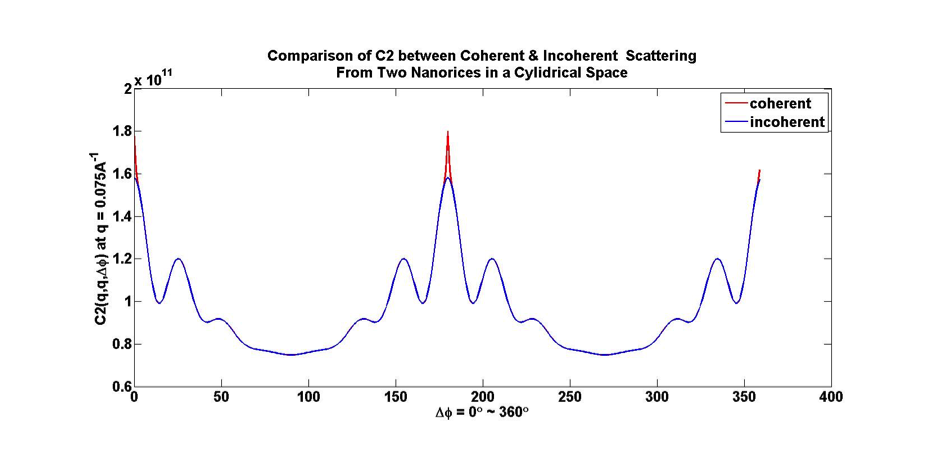
\includegraphics[width=1\textwidth]{kimplot}
\caption{Coherent peaks in (in red) in the correlations from incoherent diffraction patterns from the contributions of two independently randomly oriented nanoparticles, because the disorder gives rise to a kind of incoherence (except for narrow regions of reciprocal space that can easily be ignored \cite{kimmedicine}}
\label{fig:kimmedicine}
\end{figure}
What we mean is that in the presence of multiple particles one needs to look at correlations between particles as a result mutual interference. Quite simply, in the presence of two particles in a source of coherent radiation such an XFEL one would expect the total intensity to be $|\sum_{j=1} F_j \exp⁡(i\vec{}q\cdot\vec{r_j})|^2$ where $F_j$ is the structure factor of the jth molecule. The exponentials give rise to a factor of $\exp⁡(i\vec{q}\cdot(\vec{r}_j-\vec{r}_k )$) which results in random phases if the particle positions are random except that as $q\rightarrow 0$, when all phase factors become zero and are thus not random. Thus over most of its range one would expect interference fringes perpendicular to $\vec{r}_j-\vec{r}_k$  if the radiation is coherent. Fortunately, for different atom pairs, these fringes are random in orientation and spacing which makes the sum of cross terms amongst different particles tend towards zero, making the radiation effectively incoherent, over most of the q range as pointed out
before. It would be of interest though if the interference fringes exist. This is precisely what is observed in Figure \ref{fig:dpkim}. 
\begin{figure}[ht]
  \centering
  \includegraphics[width=0.9\textwidth]{dpkim}
\caption{Two particles illuminated simultaneously. If the radiation is coherent, one will see interference fringes, which will average out of there are many particles of random position.}
\label{fig:dpkim}
\end{figure}

While on individual diffraction patterns, fringes due to interference between the two particles are visible, the randomness of particle positions means that on different diffraction patterns these fringes will be in random directions and of random spacings. Consequently. when one adds contributions from different particles of random positions, the fringes essentially average out and it is if the sum is incoherent. That is, it is as if one were summing patterns like that in the bottom left above. Due to the randomness of the phases one may ignore the second summation over most of the $q$ range and therefore over most of the range one obtains what one would be equivalent of the incoherent sum $\sum_{j} I_j$ where $I_j$ is the intensity scattering contribution from particle $j$. Thus the total intensity reduces to a sum of intensity contributions from particle $j$, as if the scattering was not coherent \cite{kimmedicine}. The only exception occurs near $\Delta \phi =0$ (see Fig. \ref{fig:kimmedicine}, and equivalently $\Delta \phi =\pi $ due to Friedel symmetry, and $\Delta \phi = 2 \phi$ (same as $\Delta \phi =0$). These peaks are due to the fact that near $\Delta \phi =0$, all scattering phases become equal (and equal to zero). Thus the assumption of random phases is no longer valid. However, the width of such a peak is of the order of $2 \pi/L$ where $L$ is the width of the coherent radiation (about $L=1000$ \AA at the LCLS). Thus $2 \pi /L$ is usually much smaller than the width of a Shannon pixel $\pi /D$ where $D$ is of the order of $50$ Ang. Thus, in calculating $B_l$  or $T_l$  by integration under the curves of $C_2$ and $C_3$, respectively, can ignore the sharp high coherent peaks and still get essentially the same result. Thus the conclusion is for the present application of the reconstruction of the electron density of a biomolecule or virus from XFEL coherent radiation, these narrow peaks can be neglected, and the previous theory \cite{saldin2009} that applies also the single particle experiments like in the Single Particle Initiative \cite{Munke} is applicable.
\begin{figure}[ht]
  \centering
  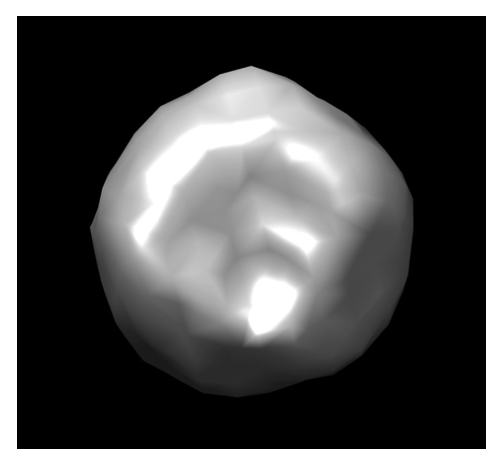
\includegraphics[width=0.7\textwidth]{kimvirus}
\caption{The rice dwarf virus (RDV) 
reconstructed from experimental data from 
the Single Particle Initiative measured in August 
2015. Note the apparent existence of internal 
genetic material, as the viruses in this 
experiment did not have the internal genetic 
material removed
}
\label{fig:kimvirus}
\end{figure}

\begin{figure}[ht]
  \centering
  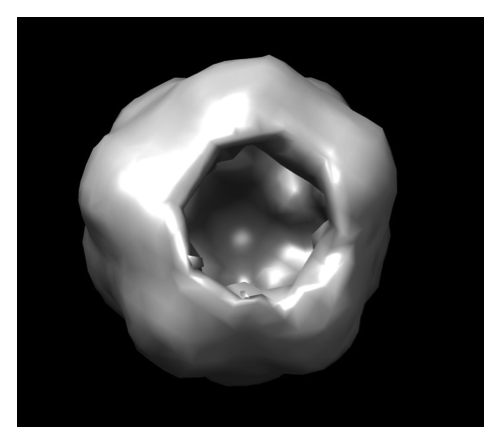
\includegraphics[width=0.7\textwidth]{kimvirus2}
\caption{
Similar image of the satellite tobacco 
necrosis virus whose structure in deposited in 
the protein data bank. This has had its internal 
genetic material removed, as revealed by the 
reconstructed image
}
\label{fig:kimvirus2}
\end{figure}

The method of angular correlations is also of great help with helical viruses \cite{PoonFiber}. In the past it has been attempted to study these entities by aligning them as in a fiber by physical means such was powerful electric fields. This has always run up against the obstacle of the entropic tendency to misalign.

Since the orientation of the reconstructed image may be chosen arbitrarily this allows an opportunity to use of the correlation method to align helical viruses computationally. It is usually assumed that the diffraction volume may be characterized by a magnetic quantum number $m=0$ if the z-axis can be taken along the helix. It turns out that even if the helices are randomly oriented in practice  merely choosing $m=0$ for the spherical harmonic components of the pair correlations $B_l$, computationally aligns the helical viruses and allows an estimate of the values of the spherical harmonic expansion coefficients of the diffraction volume \cite{PoonFiber}. Even if this is regarded as an approximation, the perturbation method we have developed for time-resolved structure \cite{pande2014} is capable of refining the values.

\begin{figure}[ht]
  \centering
  
\includegraphics[width=0.5\textwidth]{kimnano}
\caption{
Single particle of nanorice 
reconstructed from diffraction patterns of two 
independently randomly oriented particles.
}
\label{fig:kimnano}
\end{figure}

A real advantage of our method over all others that have been proposed for this problem is that it reconstructs the image from its correlations, Since the angular correlations of randomly oriented particles are identical, one can reconstruct an image of a single particle from an experiment consisting of multiple randomly oriented particles. Since the angular correlations are the same, independent of particle orientations, a corollary is that it may be reconstructed in any orientation. In general, an orientation is chosen to be consistent with the representation of the particle. An image of a single particle of nanorice reconstructed from diffraction patterns of two randomly oriented particles is shown next. 
In the case of a helical virus or a particle of nanorice, the diffraction volume is assumed to be azimuthally symmetric and m=0 is the only permitted component of the magnetic quantum number. (It should be emphasized that this is only possible because of the property of angular correlations as being the same independent of the particle orientation.)

With a focal spot of 1000 Angstrom, it is quite hard to focus on a single particle, and most diffraction patterns of proteins will probably be from multiple particles. It is true that one may remove diffraction patterns from multiple particles by so-called hit finder methods. But this is only at the expense of hit rate, as we have commented earlier 

It should be mentioned that, as currently formulated, the quantities $B_l$ and $T_l$ derived from $C_2$ and $C_3$, respectively, depend only on the azimuthal quantum number $l$. whereas the general the spherical harmonic expansion coefficients of the diffraction volume are characterized by both $l$ and the magnetic quantum number $m$. Consequently, it was proposed for both icosahedral and helical viruses that one uses the known symmetry properties for deducing the value of $m$ \cite{kam1978}. 

Ideally of course one may need to apply this method to completely non-symmetric particles. It has recently been shown to be possible to obtain spherical harmonic coefficeints $I_{lm}(q)$ characterized by particular values of $m$ by using the fact the so-called 3-point triple correlations. One first calculates the $I_{m}(q)$ coefficients of a circular harmonic expansion of the projections the structure using the method of Kurta et al. \cite{kurta} and Pedrini et al. \cite{pedrini}. Of course as one goes to lower X-ray energies one can exploit the increasingly curved nature of the Ewald sphere to get information on the $I_{lm}(q)$ coefficients of the 3D diffraction volume by an experiment like one on a “black-lipid membrane”. This will be no problem for membrane proteins which like to live within a membrane anyway. Since one of the stated aims of XFEL work is to determine the structure of hard-to-crystallize membrane proteins this a fulfillment of one of the original  aims of the construction of a nearly billion dollar XFEL.

We should also mention here other advantages of an angular momentum method particularly for icosahedral structures. Of the angular momenta $l$, while $l=0$ obviously has icosahedral symmetry, the next higher value of $l$ consistent with this symmetry is $l=6$. Consequently, if $B_l$ values are found from experimental data, the lower $l$ values should be dominated by $l=0$ and $l=6$. Thus even without an assumption of icosahedral symmetry one can get some indication of such symmetry form the experimental data even without a reconstruction of the particle’s image in real space. An example of such a calculation is shown below.

\begin{figure}[ht]
  \centering
  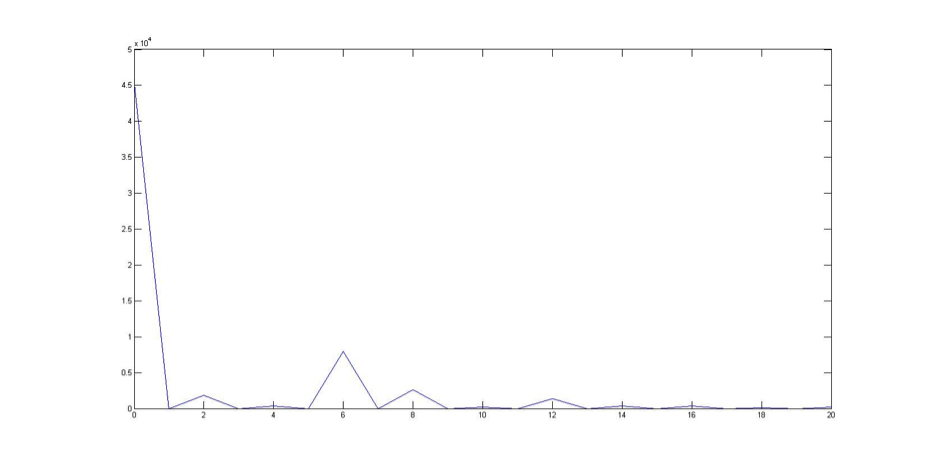
\includegraphics[width=1\textwidth]{kimBl}
\caption{
Calculation of the values of $B_l$ from experimental diffraction data from the rice dwarf virus without any symmetry assumption. This is dominated by $l=0$ and $l=6$,  a signature of icosahedral symmetry.
}
\label{fig:kimBl}
\end{figure}

Another advantage concerns the values of the intensity in the beam stop. There are less and less angular momenta as the scattering angle is reduced, In fact it can be shown that the maximum value of $l$ associated the outer edge of the beam stop is about 5. Since the maximum angular momentum associated with a given radius on a diffraction pattern is proportional to the radius and given that fact that the next lower angular momentum value consistent with icosahedral symmetry is $l=0$ one can estimate the intensity inside the beam stop if one has an analytic expression of the intensity that is angularly symmetric. In fact the known analytic form of the intensities from a uniform sphere of scattering matter is angularly symmetric, and it can be assumed to be the analytic extension of the computed intensities at higher scattering angle. This can be used to extend some of the intensities into the beam stop provided one ensures that the radial part of the data are continuous between the outer computational part and the inner analytic part. Indeed flipping-based phasing algorithms \cite{oszlanyi2004,oszlanyi2005} are often  very sensitive to the extent of the beam stop, and the extension of the data by this means is often of great help with a phasing algorithm.

%------
%Determination of molecular shape function,
%keeping all shape constant function
%Only vary the boundary
%Only use information of B zero
%The I0 enough for determinining the shape
%minimizing cost function
%I0 is independence of angular momemtun block
%------
%Time resolved structure,
%Two different structure,  
%----
%single axis random orientation
%the purpose to get the projected electron density 
%can be used to obtain nanorod 
